\documentclass[a4paper,usenames,dvipsnames]{article}

\usepackage{fullpage} % Package to use full page
\usepackage{parskip} % Package to tweak paragraph skipping
\usepackage{tikz} % Package for drawing
\usepackage{amssymb,amsmath,amsthm}
\usepackage{hyperref}
\usepackage{enumerate}
\usepackage{listings}
\usepackage{enumitem}
\usepackage{xspace}
\usepackage{colortbl}
\usepackage{xcolor}
\usepackage{kpfonts}

%\newcommand{\reed}[1]{\relax}
%\newcommand{\eric}[1]{\relax}
%\newcommand{\christian}[1]{\relax}
%\newcommand{\philipp}[1]{\relax}
%\newcommand{\Fix}[1]{\relax}
\newcommand{\reed}[1]{{\color{magenta}\bfseries [#1]}}
\newcommand{\eric}[1]{{\color{green}\bfseries [#1]}}
\newcommand{\christian}[1]{{\color{orange}\bfseries [#1]}}
\newcommand{\philipp}[1]{{\color{blue}\bfseries [#1]}}
\newcommand{\Fix}[1]{{\color{red}\bfseries [#1]}}
\newcommand{\Comment}[1]{}
\newcommand{\Space}[1]{}
\newcommand{\Num}[1]{#1}

\newcommand{\term}[1]{\emph{#1}}

\newcommand{\Free}{\textbf{Free}}

\newcommand{\evaluates}{\Downarrow}

\newcommand{\R}{\mathbb{R}}
\newcommand{\Q}{\mathbb{Q}}
\newcommand{\Z}{\mathbb{Z}}
\newcommand{\N}{\mathbb{N}}

\newcommand{\join}{\wedge}
\newcommand{\meet}{\vee}
\newcommand{\proves}{\vdash}

\newcommand{\dom}{\text{dom}~}

\newcommand{\proj}{\text{proj}}

\newcommand{\implicits}{\texttt{implicit}}
\newcommand{\params}{\texttt{params}}
\newcommand{\nonvar}{\texttt{nonvar}}

\newcommand{\tand}{\ensuremath{~\text{and}~}}
\newcommand{\tor}{\ensuremath{~\text{or}~}}
\newcommand{\twhere}{\ensuremath{~\text{where}~}}
\newcommand{\tif}{\ensuremath{~\text{if}~}}
\newcommand{\tsuchthat}{\ensuremath{~\text{s.t.}~}}
\newcommand{\owise}{\ensuremath{~\text{otherwise}~}}

\newcommand{\brackets}[3]{\ensuremath{{\left#1 {#3} \right#2}}}
\newcommand{\parens}[1]{\brackets{(}{)}{#1}}
\newcommand{\angles}[1]{\brackets{<}{>}{#1}}
\newcommand{\curlys}[1]{\brackets{\{}{\}}{#1}}
\newcommand{\squares}[1]{\brackets{[}{]}{#1}}

\newcommand{\bnfdef}{\ensuremath{\Coloneqq}}
\newcommand{\bnfalt}{\ensuremath{\mid}\xspace}

\newcommand{\inferred}{\texttt{Inferred}}
\newcommand{\prop}[1]{#1 ~ \text{prop}}
\newcommand{\typ}[1]{\text{typ}\parens{#1}}

\theoremstyle{definition}
\newtheorem{definition}{Definition}[section]
\theoremstyle{remark}
\newtheorem{remark}[definition]{Remark}
\theoremstyle{remark}
\newtheorem{example}[definition]{Example}
\theoremstyle{plain}
\newtheorem{theorem}[definition]{Theorem}
\newtheorem{conjecture}[definition]{Conjecture}

\lstdefinelanguage{pecan}{
	keywords=[1]{forall, exists, max, min, sup, inf, are, is, if, then, match, with, case, end, let, be, in, else, iff},
	keywordstyle=[1]\color{blue}\bfseries,
	keywords=[2]{false, true, sometimes},
	commentstyle=\color{CadetBlue}\textit,
	stringstyle=\color{ForestGreen}, % string literal style
	keywordstyle=[2]\color{orange}\bfseries,
	keywords=[3]{assert_prop,Structure,defining,Theorem,Prove,Example,Alias,Restrict,Define,Display,Execute,load,shuffle,import,save_aut,save_aut_img,that,context,end_context,forget,shuffle,shuffle_or,using,of},
	keywordstyle=[3]\color{teal}\bfseries,
	keywords=[4]{@annotation,@postprocess,@no_simplify,@simplify,@simplify_states,@simplify_edges},
	keywordstyle=[4]\color{purple}\bfseries,
	literate=%
	    {\#}{{{\color{teal}\bfseries\#}}}1
	    {+}{{{\color{red}+~}}}1
	    {-}{{{\color{red}-~}}}1
        {:=}{{{\color{red}:=~}}}1
        {..}{{{\color{red}..~}}}1
        {\{}{{{\color{red}\{}}}1
        {\}}{{{\color{red}\}}}}1
        {|}{{{$\color{red} \lor~$}}}1
        {*}{{{\color{red}*~}}}1
        {:}{{{\color{red}:~}}}1
        {>}{{{\color{red}>~}}}1
        {<}{{{\color{red}<~}}}1
        {<=>}{{{$\color{red}\Leftrightarrow~$}}}1
        % <= conflicts with <=> as iff, so I commented it out because it's more importnat that <=> not look weird (it becomes \leq > with the following line).
        % But might as well keep something, so I keep \iff
        % {<=}{{{$\color{red} \leq$}}}1
        % Also got rid of >= for consistency.
        % {>=}{{{$\color{red} \geq$}}}1
        {.}{{{\color{red}.~}}}1
        {&}{{{$\color{red} \land~$}}}1
        {!}{{{$\color{red}\lnot~$}}}1
        {!=}{{{$\color{red} \neq$}}}1
        {=}{{{\color{red}=~}}}1
        {exists }{{{$\color{red}\exists$}}}1
        {forall }{{{$\color{red}\forall$}}}1,
    sensitive=false, % keywords are not case-sensitive
    morecomment=[l]{//}, % l is for line comment
    morecomment=[s]{/*}{*/}, % s is for start and end delimiter
    morestring=[b]", % defines that strings are enclosed in double quotes
    showstringspaces=false
}

\lstnewenvironment{pecan}
  {
    \lstset{
        language=pecan, 
        basicstyle=\small\ttfamily, 
        mathescape=true
        }
  }
  {
  }

\lstnewenvironment{pecan_output}
  {
    \lstset{
        basicstyle=\small\ttfamily,
        mathescape=true
        }
  }
  {
  }

\newcommand{\pecaninline}[1]{\lstinline[language=pecan,basicstyle=\small\ttfamily,mathescape]{#1}}


\usepackage[
backend=biber,
style=numeric,
sorting=nty]{biblatex}

\addbibresource{biblio.bib}

\title{Building a Theorem Prover}

\author{
Authors: Reed Oei, Eric Ma \\
Graduate Mentor: Christian Schulz \\
Faculty Advisor: Philipp Hieronymi \\
}
\date{May 15, 2020}

\begin{document}

\maketitle

\section{Introduction}
An \textbf{automated theorem prover} is a program that takes a statement and \emph{decides} (i.e., proves or disproves) it. 
Theorem provers can be very useful: computers are reliable, and they never get tired or bored, allowing us to quickly explore new ideas.
Though it is impossible to decide \emph{all} statements, we can still use theorem provers to solve many interesting problems. 

Pecan is an automated theorem prover that we developed which uses B\"uchi automata to represent logical predicates.
Several notable features of Pecan include: (i) a completely automatic theorem proving process for statements expressable with B\"uchi automata; (ii) automatic counterexample generation: because automata-based theorem proving is constructive, we can generate counterexamples of any false statement given to Pecan; (iii) support for custom numeration systems and \term{automatic sequences} (sequences that can be calculated by an automaton).
Finally, because B\"uchi automata allow Pecan to work with infinitely long inputs, we can automatically prove theorems that previous systems, such as Walnut~\cite{walnut}, were unable to even express, as they only use finite automata.

\section{Background}

Let $\Sigma^*$ denote the set of finite words on the alphabet $\Sigma$, let $\Sigma^+$ denote the set of nonempty finite words on the alphabet $\Sigma$, and let $\Sigma^\omega$ denote the set of $\omega$-words on the alphabet $\Sigma$.

A \term{finite automaton} is a ``machine'' that accepts some \term{finite word}, or string of letters, such as ``abc.''
We say a finite automaton accepts a language $L(\mathcal{A})$ if and only if every string in the language is accepted by the automaton and every string not in the language is rejected by it.
They can be represented as a \emph{finite} collection of \term{states} and \term{transitions}.

Finite automata have nice closure properties: we can combine them using first-order logic operations, because they are closed under intersection, union, complementation, and projection.
Therefore, there is an algorithm that can decide any statement expressed solely in terms of first order logic operations and properties defined by finite automata.

\begin{theorem}{\cite{aut_theory}}
    Let $\mathcal{A}$ and $\mathcal{B}$ be two finite automata.
    Then we can construct automata accepting the languages $L(\mathcal{A}) \cap L(\mathcal{B})$, $L(\mathcal{A}) \cup L(\mathcal{B})$, and $L(\mathcal{A})^c$.
\end{theorem}

For the quantifiers $\forall$ and $\exists$, we define automata accepting multiple inputs. 
\begin{definition}
    An automaton $\mathcal{A}$ accepts a pair of words $ (x_1x_2\dots x_n, y_1y_2\dots y_n)$ if it accepts the word $(x_1,y_1)(x_2,y_2)\dots(x_n,y_n)$.
\end{definition}

We can generalize this definition to $n$-tuples in the natural way.

\begin{theorem}\cite{aut_theory}
    If $\varphi(x,y)$ is a predicate with two inputs, and automaton $\mathcal{A}$ over an alphabet $\Sigma$ accepts pairs of words $(x, y)$ that makes $\varphi(x, y)$ true then we can construct an automaton which accepts words that makes $\varphi'(y) = \exists x \in \Sigma. \varphi(x,y)$ true.
\end{theorem}

Therefore, we can combine predicates using first-order quantifiers and construct the automaton associated with the predicate.

\textbf{B\"uchi Automata} are an extension of the standard finite automata to infinite inputs.
A B\"uchi automaton accepts an infinite word $w \in \Sigma^\omega$ if the run of the automaton on the word $w$ visits an accepting state infinitely many times~\cite{aut_theory}.
Importantly, the languages that B\"uchi automata define are closed under intersection, union, projection, and complementation, and emptiness checking is decidable \cite{aut_theory}.

\section{Examples}

Below are some example uses of Pecan, showing it is useful in several different situations.

\subsection{The Chicken McNugget Problem}

\begin{quote}
    What is the greatest number of chicken nuggets that cannot be ordered using only boxes of 6, 9, and 20?
\end{quote}

We call all such numbers \textbf{non-purchasable}, and we can define them in Pecan as follows:

\begin{pecan}
Restrict n,m,a,b,c are binary.
n is purchasable := n is binary & existsa,b,c. n = 6*a + 9*b + 20*c
\end{pecan}

We can then define the largest non-purchasable number as:
\begin{pecan}
largest(n) := n = max { m : !purchasable(m) }
\end{pecan}

\begin{figure}
    \centering
    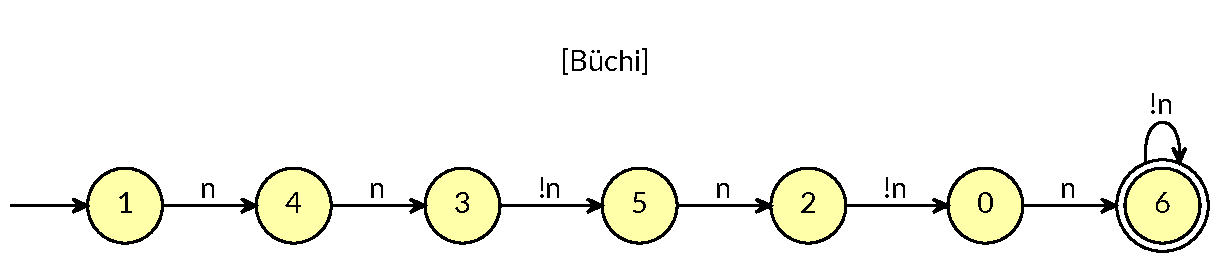
\includegraphics[width=\textwidth]{images/largest_not_purchasable.pdf}
    \caption{The B\"uchi automaton representing \pecaninline{largest(n)}, which accepts $110101_2$ ($43$ in base 10) in least significant digit first representation.}
    \label{fig:largest_non_purchasable}
\end{figure}

Pecan produces the automaton in Figure~\ref{fig:largest_non_purchasable}, which we can decode manually and see that it accepts only $43$.
We can also ask Pecan to show us what numbers \pecaninline{largest} accepts, and it will automatically perform the necessary conversions.
In this case, there is only one accepted number, so the ``example'' is the answer we're looking for.
\begin{pecan}
Example using natFormat of { largest(n) }. // Prints [(n,43)]
\end{pecan}

\subsection{The Thue-Morse Word}

We now turn to \textbf{automatic sequences}, words defined by automata, starting with the Thue-Morse word, $T$. 
The $n$-th digit of the Thue-Morse word, $T[n]$, is $1$ if the binary representation of $n$ has an odd number of $1$'s, and $0$ otherwise.
The Thue-Morse word starts with: $01101001100101101001011001101001\ldots$.

\begin{definition}
    A word $w$ is a \textbf{square} if it is of the form $w = xx$ for some word $x$.
    Similarly, $w$ is a \textbf{cube} if it is of the form $w = xxx$ for some word $x$.
\end{definition}

\begin{theorem}
    The Thue-Morse word does not contain any cubes.
\end{theorem}

Below is a Pecan definition of cubes in the Thue-Morse word and the theorem we would like to prove.
\begin{pecan}
Restrict i,j,n are binary.
square(i, n) := n > 0 & T[i..i+n] = T[i+n..i+2*n]
cube(i,n) := square(i, n) & square(i+n, n)
Theorem ("T does not contain cubes", { !(existsi,n. cube(i,n)) }).
\end{pecan}

\begin{theorem}
    There are no overlapping squares, i.e., words of form $0x0x0$ or $1x1x1$ for some nonempty word $x$. 
\end{theorem}
\begin{proof}
    We can check it by running the following Pecan commands.
\begin{pecan}
Theorem("There are no overlapping squares in the Thue-Morse word."
    { !(existsi,n. n > 0 & square(i,n) & T[i] = T[i+2*n]) }).
\end{pecan}
    Pecan verifies the theorem.
\end{proof}

\begin{definition}
    $p > 0$ is a \emph{period} of a word $w$ if $w$ is of the form $a_0 a_1 \cdots a_{p-1} a_0 a_1 \cdots a_n$; the smallest period of a word is its \emph{least period}.
\end{definition}

\begin{theorem}
    Every positive integer $p$ is the least period of some subword of the Thue-Morse word.
\end{theorem}
\begin{pecan}
p is period(i,j) := p > 0 &
    forallk. if i <= k & k < j-p then T[k]=T[k+p]
Prove that {
    forallp. if p > 0 then 
        existsi,j. p = min { m : period(i,j,m) }
}.
\end{pecan}

We can prove many more theorems about the Thue-Morse word using Pecan, but other automated theorem provers, such as Walnut, are also capable of doing so.
Therefore, we move on to other automatic sequences which Pecan is uniquely capable of reasoning about because of it's use of B\"uchi automata.

\section{Sturmian Words}
A \textbf{cutting sequence} for a curve is a sequence of $0$'s and $1$'s, corresponding to when the line crosses vertical and horizontal grid lines, respectively.
\textbf{Characteristic Sturmian words} are infinite binary sequences defined by the cutting sequence of $y = \alpha x$ for some irrational $\alpha \in (0,1)$ in the Cartesian plane.
The characteristic Sturmian word with slope $\alpha$ is written $C_{\alpha}$.
Figure~\ref{fig:fib_word} shows the characteristic Sturmian word with slope $\frac{1}{\phi}$, which begins $0100101001\ldots$.

\begin{figure}
	\centering
    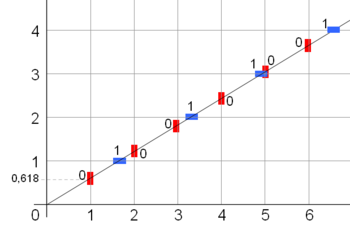
\includegraphics[width=0.5\textwidth]{images/Fibonacci_word_cutting_sequence.png}
    \caption{Characteristic Sturmian word with slope $\frac{1}{\phi}$}
    \label{fig:fib_word}
\end{figure}

Sturmian words are \term{automatic sequences} meaning that there are automata which calculate their $n$-th digit given the number $n$ in special numeration systems called \term{Ostrowski numeration systems}, based on the continued fraction of the slope $\alpha$ of the corresponding line. 
With the addition automaton for general Ostrowski numeration systems, we are able to use Pecan to \textbf{automatically prove} properties about Sturmian words. 

\subsection{Theorems about Sturmian Words}

There are many interesting properties of Sturmian words, and we can use Pecan to automatically prove many of these.

\begin{definition}
    A word is \term{eventually periodic} if it is of the form $abbbbb \ldots$ for some subwords $a$ and $b$.
    For example, the word $0.1024545454545\ldots$ is eventually periodic, with repeating part $45$.
\end{definition}

\begin{theorem}
    Sturmian words are not eventually periodic.
\end{theorem}
\begin{proof}
    In Pecan, we can write this statement as:
    
    \begin{pecan}
    eventually_periodic(a, p) := 
        p > 0 & existsn. foralli. if i > n then C[i] = C[i+p]
    Theorem ("Sturmian words are not eventually periodic", 
    { foralla,p. if p > 0 then !eventually_periodic(a,p) }).
    \end{pecan}
    
    Pecan then confirms the theorem is true for us.
\end{proof}
    
The automata have hundreds of states, and it's nearly impossible to understand them by looking at pictures of them, so we omit them here.

\begin{definition}
    A word is a palindrome if reversing it gives the same word (e.g., ``racecar'' or ``0110'').
\end{definition}

\begin{theorem}
All Sturmian words contain palindromes of every length $n$; furthermore, if $n$ is even then there is exactly one palindrome, and if $n$ is odd there are exactly two.
\end{theorem}
\begin{proof}
Using Pecan, we first define a palindrome, then we define the first occurrence of each palindrome, giving us a unique position for each palindrome of each length, and finally we ask Pecan to prove the theorem.
\begin{pecan}
palindrome(a,i,n) :=
    forallt. if t < n then C[i + t] = C[i+n-1-t]
first_palindrome(a,i,n) := palindrome(a,i,n) & 
    forallj. if j > 0 & C[j..j+n] = C[i..i+n] then i <= j
\end{pecan}
    
Finally, we state the theorem and ask Pecan to prove it. 
Pecan confirms the theorem is true.

\begin{pecan}
Prove that { foralla,n. (
if n is even then 
    existsi. forallj. first_palindrome(a,j,n) iff i=j
) & (
if n is odd then
    existsi,j. i!=j & forallk. first_palindrome(a,k,n) iff (i=k | j=k)
)}.
\end{pecan}
\end{proof}

These examples highlight Pecan's ability to quantifying over uncountable sets of strings, something that previous theorem provers with a similar approach, such as Walnut, were unable to do.
This ability allows us to state and prove theorems about \emph{all} Sturmian words, instead of just individual Sturmian words.

Pecan is capable of proving many more theorems about Sturmian words, and we are still exploring what exactly Pecan is capable of proving.
Below is a list of many more theorems that we are able to automatically prove.
It is interesting to note that several of these theorems have been proven in prior work with the use of complicated techniques, but Pecan is able to prove the same theorems automatically.
Furthermore, Pecan is able to not only prove that certain subwords exist, but also provide an automaton describing the exact locations of all subwords with the property given the slope of the Sturmian word.
Note that the exact predicates and many of the intermediate automata are available in the following GitHub repository: \url{https://github.com/ReedOei/SturmianWords}.

\begin{definition}
    A finite subword $x$ of a (finite or $\omega$) word $w$ is a \term{$n$-th power} if $x = y^n$ for some finite word $y$.
    We call a $2$nd power a \term{square}, and a $3$rd power a \term{cube}.
    
    A word that does not contain $n$-th powers is called \term{$n$-th power free} (or \term{square-free}, \term{cube-free} when appropriate).
\end{definition}

\begin{theorem}
    Sturmian words contain squares.
\end{theorem}

We reprove the following theorem from \autocite[Proposition 4.1]{PELTOMAKI2015886} and \autocite[Theorem 1]{DAMANIK2003377}.
\begin{theorem}
    If $n$ is the order of a power in $C_{\alpha}$, then $n = q_{n,\ell}$ for some $n$ and $\ell$; that is, $n$ is the denominator of a semiconvergent of $\alpha$.
\end{theorem}

Sturmian words have the interesting property that they start with arbitrarily long squares (\autocite[Theorem 1]{Dubickas2009}).

\begin{theorem}
    All Sturmian words start with arbitrarily long squares.
\end{theorem}

The following two theorems are consequences of \autocite[Theorem 4]{DAMANIK2003377}, which we can prove using Pecan.
\begin{theorem}
    All Sturmian words contain cubes.
\end{theorem}

\begin{theorem}
    A Sturmian word starts with arbitrarily long cubes if and only if its continued fraction is not eventually 1.
\end{theorem}

\begin{theorem}
    If $\alpha \in (0,1)$ is not eventually one, then $C_{\alpha}$ contains a fourth power.
\end{theorem}

\begin{definition}
    A word $w$ is called \term{mirror-invariant} if for every factor $x$ of $w$, the word $x^R$ is also a factor of $w$.
\end{definition}

We can recover the following proposition (\autocite[Proposition 2.1.19]{zbMATH01737190}):
\begin{theorem}
    All Sturmian words are mirror-invariant.
\end{theorem}

\begin{definition}
    A word $x$ is a palindrome if $x = x^R$.
\end{definition}
\begin{theorem}
    All Sturmian words start with arbitrarily long palindromes.
\end{theorem}

\begin{definition}
    A word $w$ is an \term{antisquare} if it is of the form $w = x \overline{x}$ for some $x$.
    The \term{order} of $w$ is $|x|$.
\end{definition}

\begin{definition}
    A word $w$ is an \term{antipalindrome} if $w = \overline{w^R}$.
\end{definition}

We can bound the possible lengths of antisquares and antipalindromes using the continued fraction's convergents.
We define $A_O : (0,1) \to \N$ such that $A_O(\alpha)$ is the maximum order of any antisquare in $C_{\alpha}$; we also define $A_L : (0,1) \to \N$ such that $A_L(\alpha)$ is the maximum length of any antisquare in $C_{\alpha}$.
Note that $A_L(\alpha) = 2A_O(\alpha)$.

Similarly, define $A_P : (0, 1) \to \N$ such that $A_P(\alpha)$ is the maximum length of any antipalindrome in $C_{\alpha}$.

\begin{theorem}
    For every $\alpha = [a_0, a_1, a_2, \ldots] \in (0,1)$, the following are true:
    \begin{enumerate}[label=(\roman*)]
        \item $A_O(\alpha) \leq a_3 q_3 + a_1 q_1$
        \item $A_P(\alpha) \leq a_3 q_3 + a_1 q_1$ 
        \item $A_L(\alpha) \leq a_5 q_5 + a_3 q_3 + a_1 q_1$
        \item $A_O(\alpha) \leq A_P(\alpha) \leq A_L(\alpha) = 2A_O(\alpha)$
    \end{enumerate}
    
    That is, the longest antipalindrome in $C_{\alpha}$ is at least as long as the largest order of an antisquare in $C_{\alpha}$, but it is shorter than the longest antisquare.
    Additionally, there are $\alpha, \beta \in (0, 1)$ for which the equality is achieved; that is, there is are $\alpha, \beta \in (0, 1)$ such that $A_O(\alpha) = A_P(\alpha)$ and $A_P(\beta) = A_L(\beta)$.
\end{theorem}

\begin{definition}
    A factor $x$ of a word $w$ is called \term{right special} (or just \term{special}) if $x0$ and $x1$ are both factors of $w$.
\end{definition}

\begin{theorem}
    The unique special factor of length $n$ is $C_{\alpha}[1..n+1]^R$.
\end{theorem}

\begin{definition}
    A factor $x$ of a word $w$ is called \term{recurrent} if it occurs infinitely often in $w$.
\end{definition}

\begin{theorem}
    For every $\alpha$, every factor of $C_{\alpha}$ is recurrent.
\end{theorem}

\begin{theorem}\label{thm:lesat-period-semiconvergent}
    If $p$ is the least period of a factor of $C_{\alpha}$, then $p$ is the denominator of a semiconvergent of $\alpha$; i.e., $p = q_{n,\ell}$ for some $n$ and $\ell$.
\end{theorem}

\begin{definition}
    A word $w$ is called \term{unbordered} if the least period of $w$ is $|w|$.
\end{definition}
We recover Lemma 8 of~\cite{Currie2009LeastPO}.
\begin{theorem}
    The least period of $C_{\alpha}[i..j]$ is the length of the longest unbordered factor of $C_{\alpha}[i..j]$.
\end{theorem}

\section{Future Work}

We hope to continue to develop Pecan in the future, to support automated reasoning about more expressive theories, and if feasible, to improve performance.
In addition, we plan to use Pecan to prove more properties of Sturmian words.
Finally, as Pecan uses B\"uchi automata, which accept infinite words, we can represent sets of real numbers using B\"uchi automata and prove properties about the real numbers; this could let us prove new theorems or explore other applications of Pecan aside from theorem proving.

\vspace*{10mm} %This will change to -5
\emph{
Support for this project was provided by the Illinois Geometry Lab and the Department of Mathematics at the University of Illinois at Urbana-Champaign.
}

\printbibliography

\end{document}
